% https://github.com/MartinThoma/LaTeX-examples/tree/master/tikz/max-pooling

\usetikzlibrary{arrows.meta}
\usetikzlibrary{decorations.pathreplacing}

\definecolor{c1}{HTML}{9ACFC6}
\definecolor{c2}{HTML}{DABBD6}
\definecolor{c3}{HTML}{CBDCB9}
\definecolor{c4}{HTML}{9AC3E1}
\definecolor{c5}{HTML}{DEBBA5}
\definecolor{c6}{HTML}{C4DDE5}
\newcommand*{\xMin}{0}%
\newcommand*{\xMax}{6}%
\newcommand*{\yMin}{0}%
\newcommand*{\yMax}{4}%

\newcommand*{\xMinR}{9.5}%
\newcommand*{\xMaxR}{12.5}%
\newcommand*{\yMinR}{1}%
\newcommand*{\yMaxR}{3}%

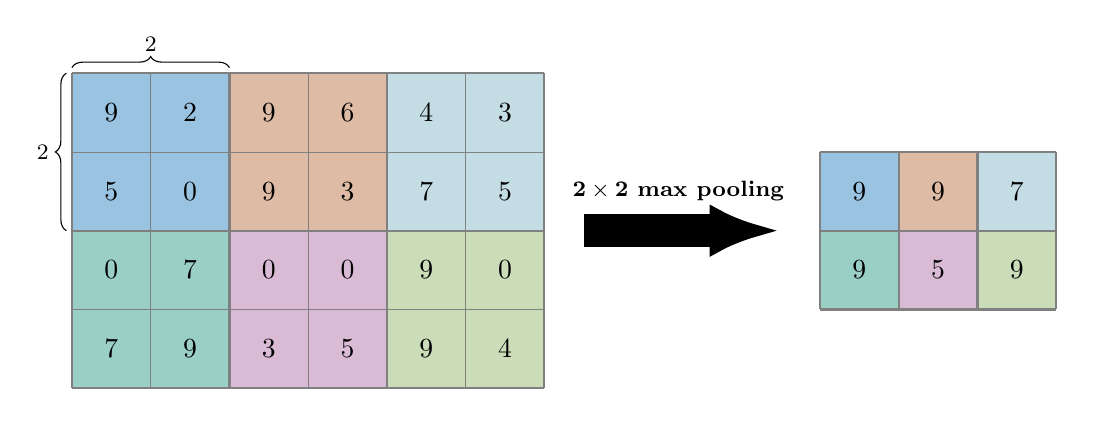
\begin{tikzpicture}
    \fill [c1] (0, 0) rectangle (2, 2);
    \fill [c2]   (2, 0) rectangle (4, 2);
    \fill [c3]  (4, 0) rectangle (6, 2);
    \fill [c4] (0, 2) rectangle (2, 4);
    \fill [c5]   (2, 2) rectangle (4, 4);
    \fill [c6]   (4, 2) rectangle (6, 4);

    \fill [c1]  (9.5, 1) rectangle (10.5, 2);
    \fill [c2]   (10.5, 1) rectangle (11.5, 2);
    \fill [c3]  (11.5, 1) rectangle (12.5, 2);
    \fill [c4]  (9.5, 2) rectangle (10.5, 3);
    \fill [c5]   (10.5, 2) rectangle (11.5, 3);
    \fill [c6]   (11.5, 2) rectangle (12.5, 3);

    \foreach \i in {\xMin,...,\xMax} {
        \draw [very thin,gray] (\i,\yMin) -- (\i,\yMax)  node [below] at (\i,\yMin) {};
    }
    \foreach \i in {\yMin,...,\yMax} {
        \draw [very thin,gray] (\xMin,\i) -- (\xMax,\i) node [left] at (\xMin,\i) {};
    }

    \foreach \i in {\xMin,2,...,\xMax} {
        \draw [thick,gray] (\i,\yMin) -- (\i,\yMax)  node [below] at (\i,\yMin) {};
    }
    \foreach \i in {\yMin,2,...,\yMax} {
        \draw [thick,gray] (\xMin,\i) -- (\xMax,\i) node [left] at (\xMin,\i) {};
    }
    \node at (0.5, 0.5) {7};
    \node at (1.5, 0.5) {9};
    \node at (2.5, 0.5) {3};
    \node at (3.5, 0.5) {5};
    \node at (4.5, 0.5) {9};
    \node at (5.5, 0.5) {4};
    %
    \node at (0.5, 1.5) {0};
    \node at (1.5, 1.5) {7};
    \node at (2.5, 1.5) {0};
    \node at (3.5, 1.5) {0};
    \node at (4.5, 1.5) {9};
    \node at (5.5, 1.5) {0};
    %
    \node at (0.5, 2.5) {5};
    \node at (1.5, 2.5) {0};
    \node at (2.5, 2.5) {9};
    \node at (3.5, 2.5) {3};
    \node at (4.5, 2.5) {7};
    \node at (5.5, 2.5) {5};
    %
    \node at (0.5, 3.5) {9};
    \node at (1.5, 3.5) {2};
    \node at (2.5, 3.5) {9};
    \node at (3.5, 3.5) {6};
    \node at (4.5, 3.5) {4};
    \node at (5.5, 3.5) {3};

    \draw[draw=black,line width=12pt,-{Latex[length=9mm]}] (6.5, 2)  -- (9,2);
    \node[font=\footnotesize\bfseries] at (7.7, 2.5) {$\mathbf{2\times 2}$ max pooling};

    \foreach \i in {\xMinR,...,\xMaxR} {
        \draw [thick,gray] (\i,\yMinR) -- (\i,\yMaxR)  node [below] at (\i,\yMinR) {};
    }
    \foreach \i in {\yMinR,...,\yMaxR} {
        \draw [thick,gray] (\xMinR,\i) -- (\xMaxR,\i) node [left] at (\xMinR,\i) {};
    }

    \node at (10, 1.5) {9};
    \node at (11, 1.5) {5};
    \node at (12, 1.5) {9};
    \node at (10, 2.5) {9};
    \node at (11, 2.5) {9};
    \node at (12, 2.5) {7};

    \draw [decorate,decoration={brace,amplitude=4pt},xshift=-2pt,yshift=0pt]
(0,2) -- (0,4) node [black,midway,xshift=-0.3cm] {\footnotesize $2$};

    \draw [decorate,decoration={brace,amplitude=4pt},xshift=0pt,yshift=2pt]
(0,4) -- (2,4) node [black,midway,yshift=+0.3cm] {\footnotesize $2$};
\end{tikzpicture}